\documentclass[12pt,a4paper]{article}
\usepackage{fontspec}
\setmainfont{Times New Roman}
\usepackage[a4paper,left=25mm,right=20mm,top=20mm,bottom=18mm]{geometry}
\usepackage{tikz}
\usetikzlibrary{positioning,arrows.meta,shapes.geometric,fit,calc}
\usepackage{xcolor}

% Custom Color Palette - Modern, high-contrast, publication-grade
\definecolor{clientbg}{RGB}{240, 246, 255}
\definecolor{clientborder}{RGB}{30, 80, 160}
\definecolor{apibg}{RGB}{236, 243, 255}
\definecolor{apiborder}{RGB}{20, 65, 145}
\definecolor{pipebg}{RGB}{248, 241, 255}
\definecolor{pipeborder}{RGB}{105, 40, 155}
\definecolor{detbg}{RGB}{238, 252, 245}
\definecolor{detborder}{RGB}{25, 125, 75}
\definecolor{clsbg}{RGB}{236, 250, 252}
\definecolor{clsborder}{RGB}{15, 120, 140}
\definecolor{databg}{RGB}{255, 248, 238}
\definecolor{databorder}{RGB}{195, 100, 20}

\tikzset{
  base/.style={
    draw,
    line width=1.1pt,
    rounded corners=5pt,
    align=center,
    inner sep=5pt
  },
  clientnode/.style={base, fill=clientbg, draw=clientborder},
  apinode/.style={base, fill=apibg, draw=apiborder},
  pipenode/.style={base, fill=pipebg, draw=pipeborder},
  detnode/.style={base, fill=detbg, draw=detborder},
  clsnode/.style={base, fill=clsbg, draw=clsborder},
  datanode/.style={base, fill=databg, draw=databorder},
  archarrow/.style={
    -{Latex[length=3mm,width=2.2mm]},
    line width=1.2pt,
    draw=black!75
  },
  biarrow/.style={
    {Latex[length=3mm,width=2.2mm]}-{Latex[length=3mm,width=2.2mm]},
    line width=1.2pt,
    draw=black!75
  },
  subtlelabel/.style={
    font=\footnotesize\bfseries,
    fill=white,
    inner sep=2pt,
    text=black!85
  }
}

\begin{document}
\pagestyle{empty}

\begin{figure}[p]
\centering
% Linewidth = 16.5cm. Center is at x=0 (-7.75cm to +7.75cm)
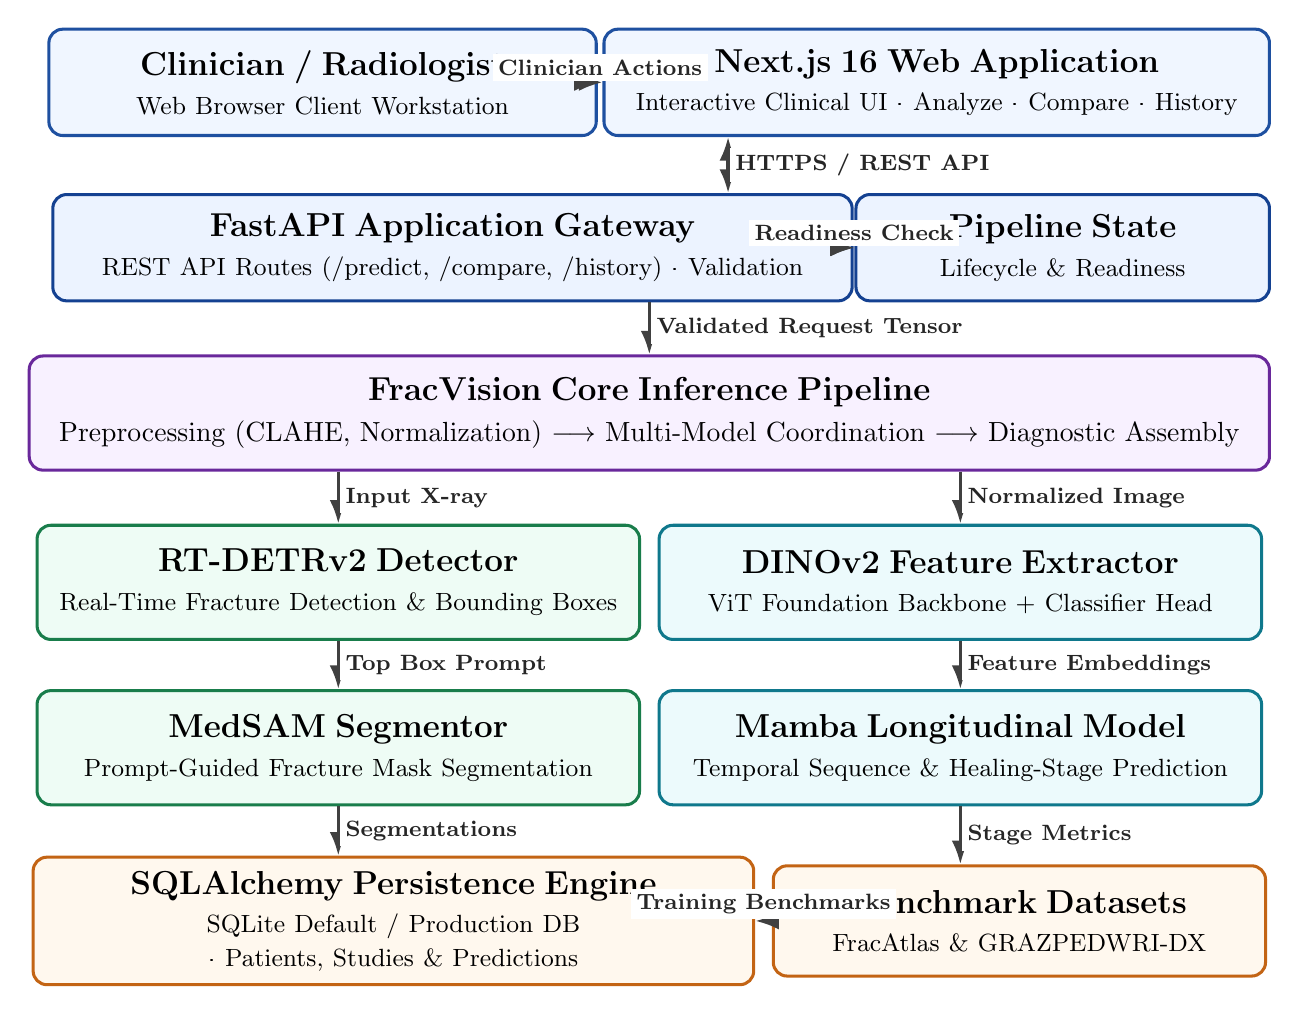
\begin{tikzpicture}

  % -------------------------------------------------------------
  % TIER 1: CLIENT & USER INTERFACE LAYER (y = 0)
  % -------------------------------------------------------------
  \node[clientnode, text width=6.6cm, minimum height=1.35cm] (user) at (-4.15, 0) {
    {\fontsize{12pt}{14pt}\selectfont\bfseries Clinician / Radiologist}\\[2pt]
    {\fontsize{9.5pt}{12pt}\selectfont Web Browser Client Workstation}
  };

  \node[clientnode, text width=8.1cm, minimum height=1.35cm] (frontend) at (3.65, 0) {
    {\fontsize{12pt}{14pt}\selectfont\bfseries Next.js 16 Web Application}\\[2pt]
    {\fontsize{9.5pt}{12pt}\selectfont Interactive Clinical UI · Analyze · Compare · History}
  };

  % -------------------------------------------------------------
  % TIER 2: BACKEND SERVICE & LIFECYCLE CONTROLLER (y = -2.1)
  % -------------------------------------------------------------
  \node[apinode, text width=9.8cm, minimum height=1.35cm] (api) at (-2.5, -2.1) {
    {\fontsize{12pt}{14pt}\selectfont\bfseries FastAPI Application Gateway}\\[2pt]
    {\fontsize{9.5pt}{12pt}\selectfont REST API Routes (/predict, /compare, /history) · Validation}
  };

  \node[apinode, text width=4.9cm, minimum height=1.35cm] (state) at (5.25, -2.1) {
    {\fontsize{12pt}{14pt}\selectfont\bfseries Pipeline State}\\[2pt]
    {\fontsize{9.5pt}{12pt}\selectfont Lifecycle \& Readiness}
  };

  % -------------------------------------------------------------
  % TIER 3: CORE INFERENCE PIPELINE (y = -4.2)
  % -------------------------------------------------------------
  \node[pipenode, text width=15.4cm, minimum height=1.45cm] (pipeline) at (0, -4.2) {
    {\fontsize{12.5pt}{15pt}\selectfont\bfseries FracVision Core Inference Pipeline}\\[3pt]
    {\fontsize{10pt}{13pt}\selectfont Preprocessing (CLAHE, Normalization) $\longrightarrow$ Multi-Model Coordination $\longrightarrow$ Diagnostic Assembly}
  };

  % -------------------------------------------------------------
  % TIER 4: PARALLEL DEEP LEARNING MODEL STREAMS
  % Left Column (x = -3.95): Detection & Segmentation
  % Right Column (x = +3.95): Classification & Progression
  % -------------------------------------------------------------
  \node[detnode, text width=7.3cm, minimum height=1.45cm] (rtdetr) at (-3.95, -6.35) {
    {\fontsize{11.5pt}{14pt}\selectfont\bfseries RT-DETRv2 Detector}\\[2pt]
    {\fontsize{9.5pt}{12pt}\selectfont Real-Time Fracture Detection \& Bounding Boxes}
  };

  \node[clsnode, text width=7.3cm, minimum height=1.45cm] (dino) at (3.95, -6.35) {
    {\fontsize{11.5pt}{14pt}\selectfont\bfseries DINOv2 Feature Extractor}\\[2pt]
    {\fontsize{9.5pt}{12pt}\selectfont ViT Foundation Backbone + Classifier Head}
  };

  \node[detnode, text width=7.3cm, minimum height=1.45cm] (seg) at (-3.95, -8.45) {
    {\fontsize{11.5pt}{14pt}\selectfont\bfseries MedSAM Segmentor}\\[2pt]
    {\fontsize{9.5pt}{12pt}\selectfont Prompt-Guided Fracture Mask Segmentation}
  };

  \node[clsnode, text width=7.3cm, minimum height=1.45cm] (mamba) at (3.95, -8.45) {
    {\fontsize{11.5pt}{14pt}\selectfont\bfseries Mamba Longitudinal Model}\\[2pt]
    {\fontsize{9.5pt}{12pt}\selectfont Temporal Sequence \& Healing-Stage Prediction}
  };

  % -------------------------------------------------------------
  % TIER 5: PERSISTENCE & BENCHMARK DATASET LAYER (y = -10.65)
  % -------------------------------------------------------------
  \node[datanode, text width=8.8cm, minimum height=1.4cm] (db) at (-3.25, -10.65) {
    {\fontsize{11.5pt}{14pt}\selectfont\bfseries SQLAlchemy Persistence Engine}\\[2pt]
    {\fontsize{9.5pt}{12pt}\selectfont SQLite Default / Production DB · Patients, Studies \& Predictions}
  };

  \node[datanode, text width=5.9cm, minimum height=1.4cm] (datasets) at (4.7, -10.65) {
    {\fontsize{11.5pt}{14pt}\selectfont\bfseries Benchmark Datasets}\\[2pt]
    {\fontsize{9.5pt}{12pt}\selectfont FracAtlas \& GRAZPEDWRI-DX}
  };

  % -------------------------------------------------------------
  % ARROWS & DATA FLOWS (Completely planar, zero crossing!)
  % -------------------------------------------------------------
  % Tier 1: User <-> Frontend
  \draw[biarrow] (user) -- node[above, subtlelabel] {Clinician Actions} (frontend);

  % Tier 1 to Tier 2: Frontend -> API (vertical at x = 1.0)
  \draw[biarrow] (frontend.south -| 1.0, 0) -- node[right, subtlelabel] {HTTPS / REST API} (api.north -| 1.0, 0);

  % Tier 2: API <-> State
  \draw[biarrow] (api) -- node[above, subtlelabel] {Readiness Check} (state);

  % Tier 2 to Tier 3: API -> Pipeline
  \draw[archarrow] (api.south -| pipeline.center) -- node[right, subtlelabel] {Validated Request Tensor} (pipeline.north);

  % Tier 3 to Tier 4: Pipeline to Detection & Classification
  \draw[archarrow] (pipeline.south -| rtdetr.center) -- node[right, subtlelabel] {Input X-ray} (rtdetr.north);
  \draw[archarrow] (pipeline.south -| dino.center) -- node[right, subtlelabel] {Normalized Image} (dino.north);

  % Inside Tier 4: Vertical Intra-Stream Pipelines
  \draw[archarrow] (rtdetr) -- node[right, subtlelabel] {Top Box Prompt} (seg);
  \draw[archarrow] (dino) -- node[right, subtlelabel] {Feature Embeddings} (mamba);

  % Tier 4 to Tier 5: Output Persistence
  \draw[archarrow] (seg) -- node[right, subtlelabel] {Segmentations} (seg |- db.north);
  \draw[archarrow] (mamba) -- node[right, subtlelabel] {Stage Metrics} (mamba |- datasets.north);

  % Datasets to DB
  \draw[archarrow] (datasets) -- node[above, subtlelabel] {Training Benchmarks} (db);

\end{tikzpicture}
\end{figure}

\end{document}
